\chapter{The \Dumux Property System}
\label{sec:propertysystem}

This section is dedicated to the \Dumux property system. First, a high
level overview over its design and principle ideas is given, then
follows a short reference and a short self-contained example.

\section{Concepts and Features of the \Dumux Property System}

The \Dumux property system was designed as an attempt to mitigate the
problems of traits classes. In fact, it can be seen as a traits system
which allows easy inheritance and any acyclic dependency of parameter
definitions. Just like traits, the \Dumux property system is a compile
time mechanism, which means that there are no run-time performance
penalties associated with it. It is based on the following concepts:
\begin{description}
\item[Property:] In the context of the \Dumux property system, a
  property is an arbitrary class body which may contain type
  definitions, values and methods. Each property has a so-called
  \textbf{property tag} which can be seen as a label with its name.
\item[Property Inheritance:] Just like normal classes, properties can
  be arranged in hierarchies. In the context of the \Dumux property
  system, nodes of the inheritance hierarchy are called \textbf{type
    tags}.
\end{description}

It also supports \textbf{property nesting} and
\textbf{introspection}. Property nesting means that the definition of
a property can depend on the value of other properties which may be
defined for arbitrary levels of the inheritance hierarchy.  The term
introspection denotes the ability to generate diagnostic messages
which can be used to find out where a certain property was defined and
how it was inherited.

\section{\Dumux Property System Reference}

All source files which use the \Dumux property system should include
the header file \texttt{dumux/ \hskip-1ex{}common/
  \hskip-1ex{}propertysystem.hh}.  Declaration of type tags and
property tags as well as defining properties must be done inside the
namespace \texttt{Dumux::Properties}.

\subsection*{Defining Type Tags}

New nodes in the type tag hierarchy can be defined using
\begin{lstlisting}[basicstyle=\ttfamily\scriptsize]
NEW_TYPE_TAG(NewTypeTagName, INHERITS_FROM(BaseTagName1, BaseTagName2, ...));
\end{lstlisting}
where the \texttt{INHERITS\_FROM} part is optional. To avoid
inconsistencies in the hierarchy, each type tag may be defined only
once for a program.

\vskip1ex\noindent
Example:
\begin{lstlisting}[basicstyle=\ttfamily\scriptsize]
namespace Dumux {
namespace Properties {
NEW_TYPE_TAG(MyBaseTypeTag1);
NEW_TYPE_TAG(MyBaseTypeTag2);

NEW_TYPE_TAG(MyDerivedTypeTag, INHERITS_FROM(MyBaseTypeTag1, MyBaseTypeTag2));
}}
\end{lstlisting}

\subsection*{Declaring Property Tags}

New property tags -- i.e. labels for properties -- are declared
using
\begin{lstlisting}[basicstyle=\ttfamily\scriptsize]
NEW_PROP_TAG(NewPropTagName);
\end{lstlisting}
A property tag can be declared arbitrarily often, in fact it is
recomended that all properties are declared in each file where they
are used.

\vskip1ex\noindent
Example:
\begin{lstlisting}[basicstyle=\ttfamily\scriptsize]
namespace Dumux {
namespace Properties {
NEW_PROP_TAG(MyPropertyTag);
}}
\end{lstlisting}

\subsection*{Defining Properties}

The value of a property on a given node of the type tag hierarchy is
defined using
\begin{lstlisting}[basicstyle=\ttfamily\scriptsize]
SET_PROP(TypeTagName, PropertyTagName)
{
  // arbitrary body of a struct
};
\end{lstlisting}
For each program, a property itself can be declared at most once,
although properties may be overwritten for derived type tags.

Also, the following convenience macros are available to define simple
properties:
\begin{lstlisting}[basicstyle=\ttfamily\scriptsize]
SET_TYPE_PROP(TypeTagName, PropertyTagName, type);
SET_BOOL_PROP(TypeTagName, PropertyTagName, booleanValue);
SET_INT_PROP(TypeTagName, PropertyTagName, integerValue);
SET_SCALAR_PROP(TypeTagName, PropertyTagName, floatingPointValue);
\end{lstlisting}

\vskip1ex\noindent
Example:
\begin{lstlisting}[basicstyle=\ttfamily\scriptsize]
namespace Dumux {
namespace Properties {
NEW_TYPE_TAG(MyTypeTag);

NEW_PROP_TAG(MyCustomProperty);
NEW_PROP_TAG(MyType);

NEW_PROP_TAG(MyBoolValue);
NEW_PROP_TAG(MyIntValue);
NEW_PROP_TAG(MyScalarValue);

SET_PROP(MyTypeTag, MyCustomProperty)
{
  static void print() { std::cout << "Hello, World!\n"; }
};
SET_TYPE_PROP(MyTypeTag, MyType, unsigned int);

SET_BOOL_PROP(MyTypeTag, MyBoolValue, true);
SET_INT_PROP(MyTypeTag, MyIntValue, 12345);
SET_SCALAR_PROP(MyTypeTag, MyScalarValue, 12345.67890);
}}
\end{lstlisting}

\subsection*{Un-setting Properties}

Sometimes some inherited properties do not make sense for a certain
node in the type tag hierarchy. These properties can be explicitly
un-set using
\begin{lstlisting}[basicstyle=\ttfamily\scriptsize]
UNSET_PROP(TypeTagName, PropertyTagName);
\end{lstlisting}
The un-set property can not be set for the same type tag, but of
course derived type tags may set it again.

\vskip1ex\noindent
Example:
\begin{lstlisting}[basicstyle=\ttfamily\scriptsize]
namespace Dumux {
namespace Properties {
NEW_TYPE_TAG(BaseTypeTag);
NEW_TYPE_TAG(DerivedTypeTag, INHERITS_FROM(BaseTypeTag));

NEW_PROP_TAG(TestProp);

SET_TYPE_PROP(BaseTypeTag, TestProp, int);
UNSET_PROP(DerivedTypeTag, TestProp);
// trying to access the 'TestProp' property for 'DerivedTypeTag' 
// will trigger a compiler error!
}}
\end{lstlisting}

\subsection*{Converting Tag Names to Tag Types}

For the C++ compiler, property and type tags are like ordinary
types. Both can thus be used as template arguments. To convert a
property tag name or a type tag name into the corrosponding type, the
macros \texttt{TTAG(TypeTagName)} and \texttt{PTAG(PropertyTagName)}
ought to be used.

\subsection*{Retrieving Property Values}

The value of a property can be retrieved using
\begin{lstlisting}[basicstyle=\ttfamily\scriptsize]
GET_PROP(TypeTag, PropertyTag)
\end{lstlisting}
or using the convenience macros
\begin{lstlisting}[basicstyle=\ttfamily\scriptsize]
GET_PROP_TYPE(TypeTag, PropertyTag)
GET_PROP_VALUE(TypeTag, PropertyTag)
\end{lstlisting}

\vskip1ex
\noindent
The first convenience macro retrieves the type defined using
\texttt{SET\_TYPE\_PROP} and is equivalent to
\begin{lstlisting}[basicstyle=\ttfamily\scriptsize]
GET_PROP(TypeTag, PropertyTag)::type
\end{lstlisting}
while the second convenience macro retrieves the value of any property
defined using \texttt{SET\_\{INT,BOOL,SCALAR\}\_PROP} and is
equivalent to
\begin{lstlisting}[basicstyle=\ttfamily\scriptsize]
GET_PROP(TypeTag, PropertyTag)::value
\end{lstlisting}

\vskip1ex\noindent
Example:\nolinebreak
\begin{lstlisting}[basicstyle=\ttfamily\scriptsize]
template <TypeTag>
class MyClass {
  // retrieve the ::value attribute of the 'NumEq' property
  enum { numEq = GET_PROP(TypeTag, PTAG(NumEq))::value }; 
  // retrieve the ::value attribute of the 'NumPhases' property using the convenience macro
  enum { numPhases = GET_PROP_VALUE(TypeTag, PTAG(NumPhases)) }; 

  // retrieve the ::type attribute of the 'Scalar' property
  typedef typename GET_PROP(TypeTag, PTAG(Scalar))::type Scalar; 
  // retrieve the ::type attribute of the 'Vector' property using the convenience macro
  typedef typename GET_PROP_TYPE(TypeTag, PTAG(Vector)) Vector;
};
\end{lstlisting}

\subsection*{Nesting Property Definitions}

Inside property definitions there is access to all other properties
which are defined somewhere on the type tag hierarchy. The node for
which the current property is requested is available via the keyword
\texttt{TypeTag}. Inside property class bodies this can be used to
retrieve other properties using the \texttt{GET\_PROP} macros.

\vskip1ex\noindent
Example:
\begin{lstlisting}[basicstyle=\ttfamily\scriptsize]
SET_PROP(MyModelTypeTag, Vector)
{
private: typedef typename GET_PROP_TYPE(TypeTag, PTAG(Scalar)) Scalar;
public: typedef std::vector<Scalar> type;
};
\end{lstlisting}


\section{A Self-Contained Example}

As a concrete example, let us consider some kinds of cars: Compact
cars, sedans, trucks, pickups, military tanks and the Hummer-H1 sports
utility vehicle. Since all these cars share some characteristics, it
makes sense to inherit those from the closest matching car type and
only specify the properties which are different. Thus, an inheritance
diagram for the car types above might look like outlined in Figure
\ref{fig:car-hierarchy}.

\begin{figure}[t]
  \centering 
  \subfloat[]{
    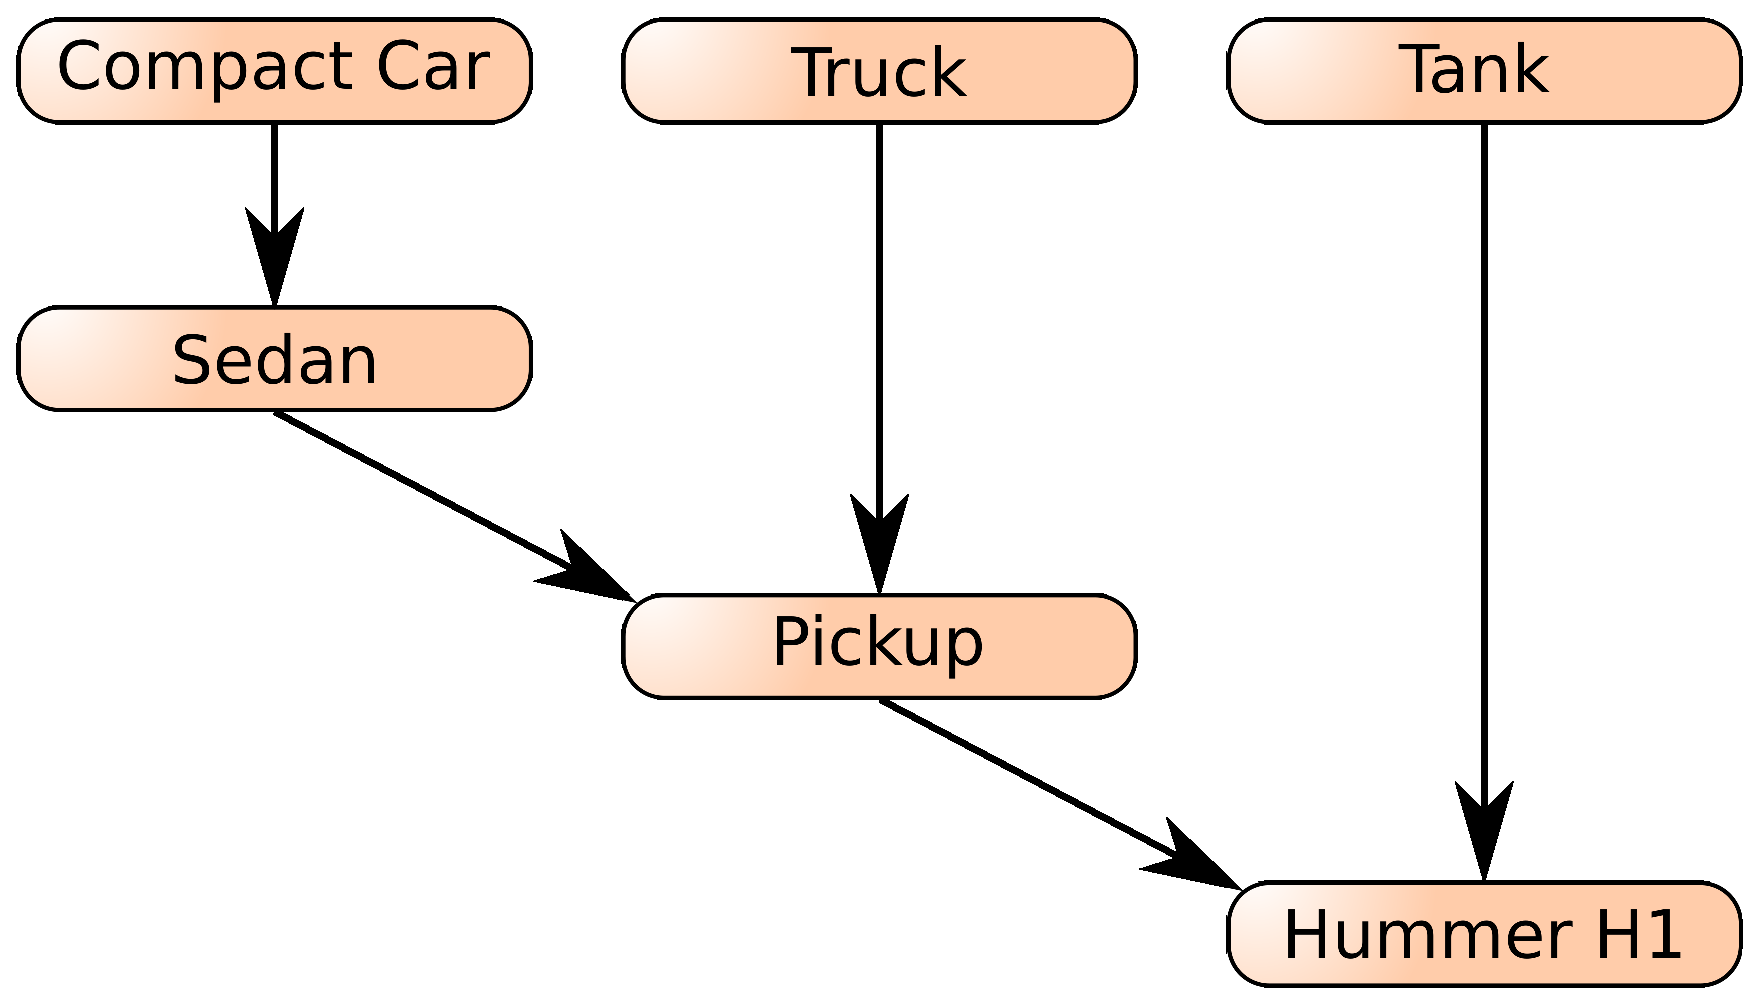
\includegraphics[width=.6\textwidth]{EPS/car-hierarchy.eps}
    \label{fig:car-hierarchy}
  }
  \subfloat[]{
    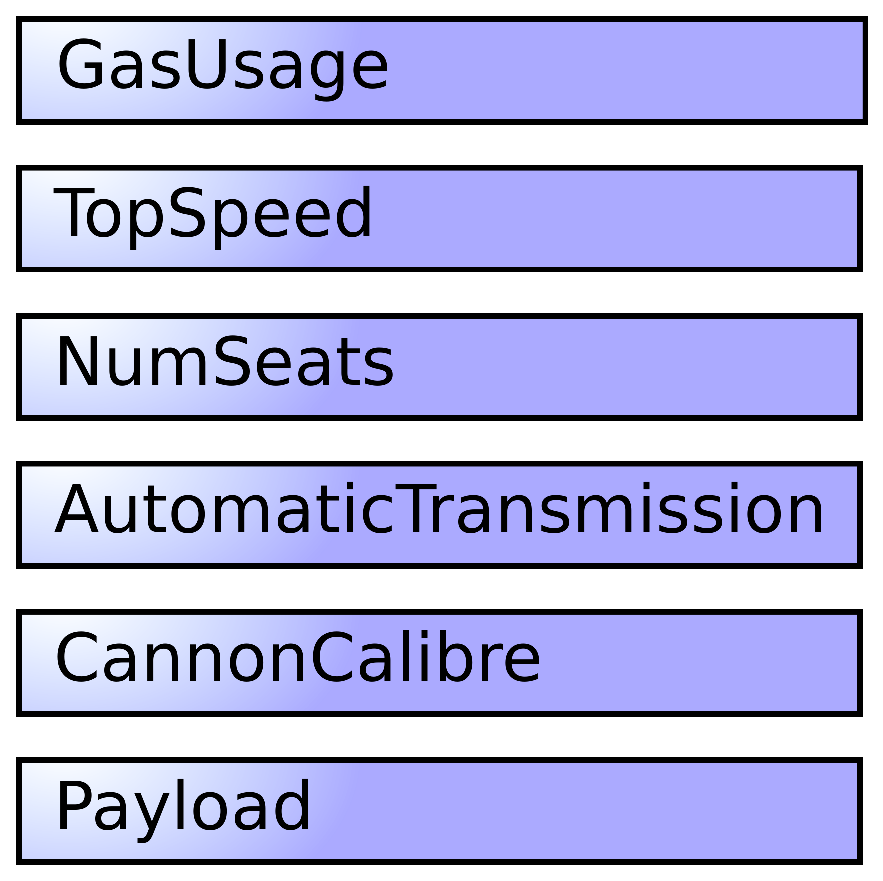
\includegraphics[width=.35\linewidth, keepaspectratio]{EPS/car-propertynames.eps}
    \label{fig:car-propertynames}
  }
  \caption{ \textbf{(a)}~~A possible property inheritance graph for
    various kinds of cars.  The lower nodes inherit from higher ones;
    Inherited properties from nodes on right take precedence over the
    properties defined on the left. ~~\textbf{(b)}~~Property names
    which make sense for at least one of the car types of (a).  }
\end{figure}

Using the \Dumux property system, this inheritance hierarchy is
defined by:
\begin{lstlisting}[name=propsyscars,basicstyle=\ttfamily\scriptsize,numbers=left,numberstyle=\tiny, numbersep=5pt]
#include <dumux/common/propertysystem.hh>
#include <iostream>

namespace Dumux {
namespace Properties {
NEW_TYPE_TAG(CompactCar);
NEW_TYPE_TAG(Truck);
NEW_TYPE_TAG(Tank);
NEW_TYPE_TAG(Sedan, INHERITS_FROM(CompactCar));
NEW_TYPE_TAG(Pickup, INHERITS_FROM(Sedan, Truck));
NEW_TYPE_TAG(HummerH1, INHERITS_FROM(Pickup, Tank));
\end{lstlisting}

Figure \ref{fig:car-propertynames} lists a few property names which
make sense for at least one of the nodes of Figure
\ref{fig:car-hierarchy}. These property names can be declared as
follows:
\begin{lstlisting}[name=propsyscars,basicstyle=\ttfamily\scriptsize,numbers=left,numberstyle=\tiny, numbersep=5pt]
NEW_PROP_TAG(TopSpeed); // [km/h]
NEW_PROP_TAG(NumSeats); // []
NEW_PROP_TAG(CanonCaliber); // [mm]
NEW_PROP_TAG(GasUsage); // [l/100km]
NEW_PROP_TAG(AutomaticTransmission); // true/false
NEW_PROP_TAG(Payload); // [t]
\end{lstlisting}

\noindent
So far, the inheritance hierarchy and the property names are completely
separate. What is missing is setting some values for the property
names on specific nodes of the inheritance hierarchy. Let us assume
the following:
\begin{itemize}
\item For a compact car, the top speed is the gas usage in $l/100km$
  times $30$, the number of seats is $5$ and the gas usage is
  $4\;l/100km$.
\item A truck is by law limited to $100\;km/h$ top speed, the number
  of seats is $2$, it uses $18\;l/100km$ and has a cargo payload of
  $35\;t$.
\item A tank exhibits a top speed of $60\;km/h$, uses $65\;l/100km$
  and features a $120\;mm$ diameter canon 
\item A sedan has a gas usage of $7\;l/100km$, as well as an automatic
  transmission, in every other aspect it is like a compact car.
\item A pick-up truck has a top speed of $120\;km/h$ and a payload of
  $5\;t$. In every other aspect it is like a sedan or a truck but if in
  doubt it is more like a truck.
\item The Hummer-H1 SUV exhibits the same top speed as a pick-up
  truck.  In all other aspects it is similar to a pickup and a tank,
  but if in doubt more like a tank.
\end{itemize}

\noindent
Using the \Dumux property system, these assumptions are formulated
using
\begin{lstlisting}[name=propsyscars,basicstyle=\ttfamily\scriptsize,numbers=left,numberstyle=\tiny, numbersep=5pt]
SET_INT_PROP(CompactCar, TopSpeed, GET_PROP_VALUE(TypeTag, PTAG(GasUsage)) * 30);
SET_INT_PROP(CompactCar, NumSeats, 5);
SET_INT_PROP(CompactCar, GasUsage, 4);

SET_INT_PROP(Truck, TopSpeed, 100);
SET_INT_PROP(Truck, NumSeats, 2);
SET_INT_PROP(Truck, GasUsage, 18);
SET_INT_PROP(Truck, Payload, 35);

SET_INT_PROP(Tank, TopSpeed, 60);
SET_INT_PROP(Tank, GasUsage, 65);
SET_INT_PROP(Tank, CanonCaliber, 120);

SET_INT_PROP(Sedan, GasUsage, 7);
SET_BOOL_PROP(Sedan, AutomaticTransmission, true);

SET_INT_PROP(Pickup, TopSpeed, 120);
SET_INT_PROP(Pickup, Payload, 5);

SET_INT_PROP(HummerH1, TopSpeed, GET_PROP_VALUE(TTAG(Pickup), PTAG(TopSpeed)));
\end{lstlisting}

\noindent
At this point, the Hummer-H1 has a $120\;mm$ canon which it inherited
from its military ancestor. It can be removed by
\begin{lstlisting}[name=propsyscars,basicstyle=\ttfamily\scriptsize,numbers=left,numberstyle=\tiny, numbersep=5pt]
UNSET_PROP(HummerH1, CanonCaliber);

}} // close namespaces
\end{lstlisting}

\noindent
Now property values can be retrieved and some diagnostic messages can
be generated. For example
\begin{lstlisting}[name=propsyscars,basicstyle=\ttfamily\scriptsize,numbers=left,numberstyle=\tiny, numbersep=5pt]
int main()
{
    std::cout << "top speed of sedan: " << GET_PROP_VALUE(TTAG(Sedan), PTAG(TopSpeed)) << "\n";
    std::cout << "top speed of truck: " << GET_PROP_VALUE(TTAG(Truck), PTAG(TopSpeed)) << "\n";

    std::cout << PROP_DIAGNOSTIC(TTAG(Sedan), PTAG(TopSpeed));
    std::cout << PROP_DIAGNOSTIC(TTAG(HummerH1), PTAG(CanonCaliber));
}
\end{lstlisting}
will yield the following output:
\begin{lstlisting}[basicstyle=\ttfamily\scriptsize,numbers=left,numberstyle=\tiny, numbersep=5pt]
top speed of sedan: 210
top speed of truck: 100
Property 'TopSpeed' for type tag 'Sedan'
  inherited from 'CompactCar'
    defined at test_propertysystem.cc:90
Property 'CanonCaliber' for type tag 'HummerH1'
  explicitly unset at test_propertysystem.cc:113
\end{lstlisting}


%%% Local Variables: 
%%% mode: latex
%%% TeX-master: "dumux-handbook"
%%% End: 
